\section{Game engine architecture}
New sections should not start with directly a subsection, rather with short section introduction. 

\subsection{Overview of architecture}
% Opisanie architektury silnika, sposobu komunikacji między komponentami, a także za co one odpowiadają.
Lorem ipsum dolor sit amet, consectetur adipiscing elit. Nam consectetur dignissim urna, a rhoncus dolor venenatis adipiscing. Phasellus viverra aliquam fringilla. Praesent mattis diam id ipsum placerat a laoreet diam tempus. Quisque eu leo ut sapien ultricies gravida ac sed turpis. Donec nibh enim, pretium a sagittis et, varius non nulla. Vivamus enim augue, condimentum eget convallis hendrerit, mattis ut lectus. Cum sociis natoque penatibus et magnis dis parturient montes, nascetur ridiculus mus. Proin semper libero augue. Praesent auctor ligula sit amet quam molestie adipiscing. Mauris vehicula congue mollis. Duis tincidunt interdum purus quis congue. Integer vel orci mauris. Curabitur rutrum tincidunt mi ut elementum. Nunc non massa nunc. Donec ultricies ipsum ac risus sollicitudin porta. Phasellus elementum odio et leo consectetur consectetur. 

Lorem ipsum dolor sit amet, consectetur adipiscing elit. Nam consectetur dignissim urna, a rhoncus dolor venenatis adipiscing. Phasellus viverra aliquam fringilla. Praesent mattis diam id ipsum placerat a laoreet diam tempus. Quisque eu leo ut sapien ultricies gravida ac sed turpis. Donec nibh enim, pretium a sagittis et, varius non nulla. Vivamus enim augue, condimentum eget convallis hendrerit, mattis ut lectus. Cum sociis natoque penatibus et magnis dis parturient montes, nascetur ridiculus mus. Proin semper libero augue. Praesent auctor ligula sit amet quam molestie adipiscing. Mauris vehicula congue mollis. Duis tincidunt interdum purus quis congue. Integer vel orci mauris. Curabitur rutrum tincidunt mi ut elementum. Nunc non massa nunc. Donec ultricies ipsum ac risus sollicitudin porta. Phasellus elementum odio et leo consectetur consectetur. 

\subsection{Components of a solution}
% Opisanie elementów z jakich się składa rozgrywka m.in.: kafelki i ich elementy, gracze, a także uwzględnione rozszerzenia gry Carcassonne.

The game Carcassone is played by placing tiles \cite{CarcassoneRules}. Each tile is represented by a set of features on it. All features are defined by their type, such as road, city, field or monastery, a modifier that modifies the calculation process, and the sides which indicate on which edges the feature is present. In this project there is only one modifier used - the shield. The engine was designed to accommodate game extensions. 

A feature's side is a byte sized value, in which each bit defines whether the feature is present on a specific half of the tile's edge as shown on Figure \ref{fig:SIDES}. Features such as roads, are represented by a whole edge formed by combining two sides e.g., the TopLeft and TopRight sides.
\begin{figure}
    \centering
    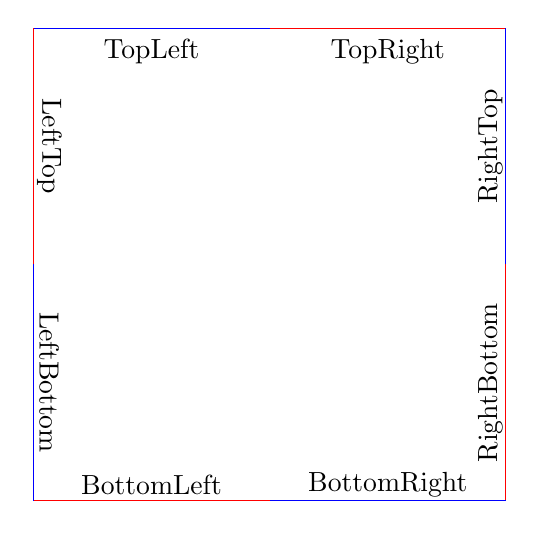
\begin{tikzpicture}
        %top line
        \draw [blue] (-3,3) -- (0,3);
        \draw [red] (0,3) -- (3,3);
        %right line
        \draw [blue] (3,3) -- (3,0);
        \draw [red] (3,0) -- (3,-3);
        %bottom line
        \draw [blue] (3,-3) -- (0,-3);
        \draw [red] (0,-3) -- (-3,-3);
        %left line
        \draw [blue] (-3,-3) -- (-3,0);
        \draw [red] (-3,0) -- (-3,3);
        
        \node at (-1.5, 2.7) {TopLeft};
        \node at (1.5, 2.7) {TopRight};
        
        \node [rotate=90] at (2.8, 1.5) {RightTop};
        \node [rotate=90] at (2.8, -1.5) {RightBottom};
        
        \node at (-1.5, -2.8) {BottomLeft};
        \node at (1.5, -2.8) {BottomRight};
        
	% czy może obrót 90stopni?
        \node [rotate=270] at (-2.8, 1.5) {LeftTop};
        \node [rotate=270] at (-2.8, -1.5) {LeftBottom};
    \end{tikzpicture}
    \caption{Side representation} \label{fig:SIDES}
\end{figure}

The tiles described do not contain information about their position or meeple placement. This information is located in the PlacedTile struct. The board is represented as a slice of placed tiles ordered by their placement, moreover it contains the used tile set, for verification whether the tile a player wants to place is legal. Additionally, board includes a city manager used for merging cities, scoring and checking for legal meeples placement in the cities.

A single game is represented by a board, shuffled deck of tiles, and players taking their turns. Each player knows their score, and the number of meeples of each type available to them.

Our solution has been designed to be modifiable by adding extensions to the game. Generalizations, such as meeple type or feature type, allow for the easy implementation of new potential features e.g., rivers.

\subsection{Execution flow}
% Opisanie wykonywanych akcji podejmowanych przez silnik gry: wylosowanie kafelka ze stosu, wyliczenie legalnych ułożeń kafelka, wybór położenia i wyliczanie punktacji za jego położenie.
Lorem ipsum dolor sit amet, consectetur adipiscing elit. Nam consectetur dignissim urna, a rhoncus dolor venenatis adipiscing. Phasellus viverra aliquam fringilla. Praesent mattis diam id ipsum placerat a laoreet diam tempus. Quisque eu leo ut sapien ultricies gravida ac sed turpis. Donec nibh enim, pretium a sagittis et, varius non nulla. Vivamus enim augue, condimentum eget convallis hendrerit, mattis ut lectus. Cum sociis natoque penatibus et magnis dis parturient montes, nascetur ridiculus mus. Proin semper libero augue. Praesent auctor ligula sit amet quam molestie adipiscing. Mauris vehicula congue mollis. Duis tincidunt interdum purus quis congue. Integer vel orci mauris. Curabitur rutrum tincidunt mi ut elementum. Nunc non massa nunc. Donec ultricies ipsum ac risus sollicitudin porta. Phasellus elementum odio et leo consectetur consectetur. 

Lorem ipsum dolor sit amet, consectetur adipiscing elit. Nam consectetur dignissim urna, a rhoncus dolor venenatis adipiscing. Phasellus viverra aliquam fringilla. Praesent mattis diam id ipsum placerat a laoreet diam tempus. Quisque eu leo ut sapien ultricies gravida ac sed turpis. Donec nibh enim, pretium a sagittis et, varius non nulla. Vivamus enim augue, condimentum eget convallis hendrerit, mattis ut lectus. Cum sociis natoque penatibus et magnis dis parturient montes, nascetur ridiculus mus. Proin semper libero augue. Praesent auctor ligula sit amet quam molestie adipiscing. Mauris vehicula congue mollis. Duis tincidunt interdum purus quis congue. Integer vel orci mauris. Curabitur rutrum tincidunt mi ut elementum. Nunc non massa nunc. Donec ultricies ipsum ac risus sollicitudin porta. Phasellus elementum odio et leo consectetur consectetur. 

\subsection{Communication within a system}
% Opisanie komunikacji pomiędzy silnikiem gry, a sieciami neuronowymi uczonymi na karcie graficznej. Aktualizacja stanu gry w zależności od akcji podejmowanych przez agenta.

The game engine is capable of handling multiple game instances, by using Go pipelines and goroutines \cite{GolangPipeline}, which allows for many agents to play and learn simultaneously. The engine provides several requests necessary for the agents, to retrieve information about the game. There are five such requests:
\begin{itemize}
    \item CloneGame - used for creating a separate clone of a game. It allows the agent to expand the game tree, and each clone can be modified by the agent, by simulating its next potential move.
    \item GetRemainingTiles - returns all available tiles that have not yet been placed. With this data, the agent can expand the game tree for each possible move that might occur. The returned tiles come with information about their probability.
    \item GetLegalMoves - returns all legal moves for a given tile. It considers where tile can be placed and where the possible meeple placement on it.
    \item GetMidGameScore - returns the information about the score for all players, calculated as if the game has just finished.
    \item PlayTurn - allows the agent to play a turn using a given tile, and modifies the game state. It returns the new state of the game 
\end{itemize}

% coś o tym że  agent może budować drzewo jak w algorytmie alphago, ale troche nie wiem jak ten akapit rozwinąć.
With these requests, the agent is capable of building its own game tree, as in the AlphaGo algorithm \cite{AlphaGoAlgorithm}.

To provide the neural network with the game state, a serialization process is required. Serialized game contains all players' statistics (meeple counts, score) and all tiles on the board. The placed tiles on the board are represented in the binary format to ensure a fixed memory size of 8 bytes. The slice of binary tiles consists of all tiles in placement order. The tiles in this array that are not yet placed are set to zero.
